\chapter{Differenzierbarkeit}
\Mark{Chapter 4.1}
$f$: $D \ra \R$ stetig dann bedeutet dies, dass $f$ in $D$ keine \ggq{Spr�nge} hat\\
$f$: $D \ra \R$ differenzierbar bedeutet, dass $f$ in $D$ keine Spr�nge und keine \ggq{Knicke} hat

\begin{fdefinition}[Differenzierbarkeit]
Die Funktion $f$: $D \ra \R$ hei�t im Punkt $x_0 \in D$ \indexb{differenzierbar}, falls der Grenzwert
\[f' (x_0) \ceq \lim_{x \ra x_0} \frac{f(x) - f(x_0)}{x - x_0}\]
existiert $(f' (x_0) \in \R)$.\\
Die Zahl $f'(x_0)$ hei�t dann \indexb{Ableitung} von $f$ an der Stelle $x_0$.\\
Die Funktion $f$: $D \ra \R$ hei�t differenzierbar in $A \subseteq D$, falls $f$ in jedem $x_0 \in A$ differenzierbar ist.
\Mark{Definition 4.1}
\end{fdefinition}
\section*{Geometrische Interpretation}
\begin{figure}[h]
\centering
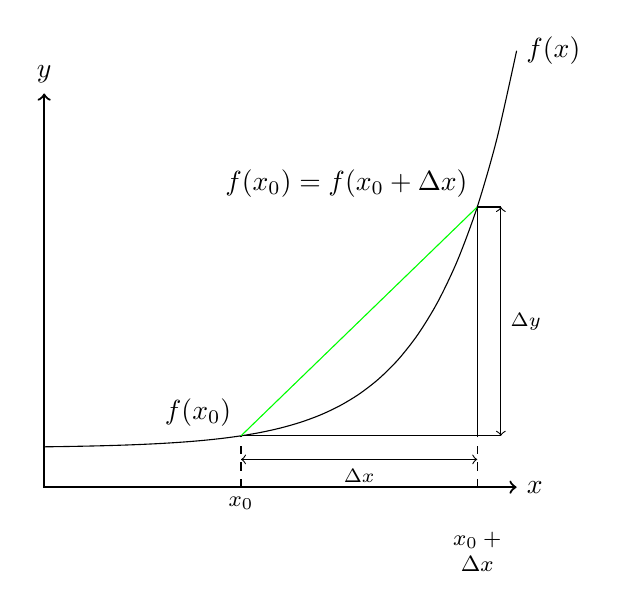
\begin{tikzpicture}[domain=0:6]
\draw[<->,thick] (0,5) node[above] {$y$} -- (0,0) -- (6,0) node[right] {$x$};
\draw plot[smooth] (\x,{exp(\x)/80 + 0.5}) node[right] {$f(x)$};
\draw (2.5,{exp(2.5)/80 + 0.5}) -- (5.5,{exp(2.5)/80 + 0.5}) -- (5.5,{exp(5.5)/80 + 0.5});
\draw[color=green] (2.5,{exp(2.5)/80 + 0.5}) node[above left, color=black] {$f(x_0)$} -- (5.5,{exp(5.5)/80 + 0.5}) node[above left, color=black] {$f(x_0) = f(x_0 + \Delta x)$};
\draw[dashed] (2.5,0) node[below] {\footnotesize{$x_0$}} -- (2.5,{exp(2.5)/80 + 0.5});
\draw[dashed] (5.5,0) node[below, text width=7mm] {\begin{center}\footnotesize{$x_0 + \Delta x$}\end{center}} -- (5.5,{exp(5.5)/80 + 0.5});

\draw[<->] (2.5,{exp(2.5)/80 + 0.2}) -- (5.5,{exp(2.5)/80 + 0.2}) node[below, midway] {\scriptsize{$\Delta x$}};
\draw (5.5,{exp(2.5)/80 + 0.5}) -- (5.8,{exp(2.5)/80 + 0.5});
\draw (5.5,{exp(5.5)/80 + 0.5}) -- (5.8,{exp(5.5)/80 + 0.5});
\draw[<->] (5.8,{exp(2.5)/80 + 0.5}) -- (5.8,{exp(5.5)/80 + 0.5}) node[right, midway] {\scriptsize{$\Delta y$}};
\end{tikzpicture}
\end{figure}
\Img{MA2-28.04.2009-IMG-1}

Mit $h = \Delta x$ stellt der Differenzenquotient
\[\frac{f(x_0 + \Delta x) - f(x_0)}{\delta x} = \frac{f(x_0 + h) - f(x_0)}{h} = \frac{\Delta y}{\Delta x} = \frac{\Delta f}{\Delta x}\]
die Steigung der Sekante (Sehne) zwischen $f(x_0)$ und $f(x_0 + \Delta x)$ dar.\\
F�r $h \ra 0$ \ac{bzw.} $\Delta x \ra 0$ geht die Sekante in die Tangente in $x_0$ �ber und Steigung der Tangente ist
\begin{align*}
f'(x_0) &= \frac{df(x)}{dx}_{x = x_0} = \frac{df}{dx}_{(x_0)} = \lim_{\Delta x \ra 0} \frac{f(x + \Delta x) - f(x_0)}{\Delta x}\\
&=\tanx{\alpha}
\end{align*}

\begin{bemerkung}
\mbox{}\par
\begin{enumerate}
\item In Anlehnung an d en Differenzenquotient $\frac{\Delta f}{\Delta x}$ nennt man $\frac{df}{dx}$ \indexb{Differenzialquotient}.
\item $h$ \ac{bzw.} $\Delta x$ muss nicht $> 0$ sein.
\item Alternative Definition der Differenzierbarkeit\\
		Sei $D \subseteq \R$ und $x_0 \in D$, so dass mindestens eine Folge $(x_n)_{n \in \N}$ mit $x_n \in D \backslash \gklamm{x_0}$ existiert mit $\lim_{n \ra \un} (x_n) = x_0$.\\
		Eine Funktion $f$: $D \ra \R$ hei�t differenzierbar in $x_0 \in D$, falls es eine Konstante $a \in \R$ und eine Funktion $r$: $D \ra \R$ mit $\lim_{x \ra x_0} r(x) = 0$ gibt, sodass
		\[f(x) = f(x_0) + a \mal (x - x_0) + r(x) \mal (x - x_0)~~x \in D\]
		In diesem Fall ist $a = f' (x_0)$

\item Die Gleichung der Tangente an $f$ in $x_0$ lautet
		\[\ub{T(f, x)}{= T(x) = T_f(x)} = f(x_0) + f' (x_0) \mal (x - x_0)\]

\item aus 3, 4 folgt, dass sich lokal (also in der N�he eines gegebenen Punktes $x_0$) der \ggq{Zuwachs} der Funktion $f$ durch den Zuwachs der Tangente $T_f$ ($a_n$ $f in x_0$) darstellen l�sst.
		\begin{align*}
		\Delta f &= f(x) - f(x_0)\\
		&= f(x_0) + f'(x_0) (x - x_0) + r(x) \mal (x - x_0) - f(x_0)\\
		&= f'(x_0) \mal (x - x_0) + r(x) \mal (x - x_0)\\
		&\approx f'(x_0) \mal (x - x_0)\\
		&= T_f(x) - T_f(x_0)\\
		\Ra& df = f'(x) dx \tx{ Differential}
		\end{align*}
		\ac{d.h.} wenn man um die Infinitesimale Gr��e $dx$ von $x_0$ weggeht, �ndert sich der Funktionswert um $df = f'(x_0) dx$
\end{enumerate}
\end{bemerkung}

\begin{beispiel}
\mbox{}\par
\begin{enumerate}
\item $f(x) = 4x - 5$\\
		Ist $f$ in $x_0 = 3$ differenzierbar?\\
		Ist $f$ in $\R$ differenzierbar?
		\begin{align*}
		\lim_{x \ra x_0} \frac{f(x) - f(x_0)}{x - x_0} &= \lim_{h \ra 0} \frac{f(x_0 + h) - f(x_0)}{h}\\
		&= \lim_{h \ra 0} \frac{\rkl{4 (x_0 + h) - 5} - (4 x_0 - 5)}{h}\\
		&= \lim_{h \ra 0} \frac{4x_0 + 4h - 5 - 4x_0 + 5}{h} = \lim_{h \ra 0} 4 = 4
		\end{align*}
		Da der Grenzwert existiert ohne dass wir den Wert von $x_0$ gebraucht h�tten, ist $f$ in ganz $\R$ differenzierbar.
\end{enumerate}
\end{beispiel}

\section{Aufgabe 4.1}
\label{sec:Differenzierbarkeit_A4_1}
Ermitteln sie die Ableitung der Funktion $f(x) = x^2$ direkt mit Hilfe der Definition

L�sung siehe \vref{sec:Differenzierbarkeit_A4_1L}.
\Solved{Link zu L�sung}

\begin{beispiel}
\mbox{}\par
\begin{enumerate}[start=2]
\item $f(x) = e^x$ gesucht $f'(x)$
		\begin{align*}
		\lim_{x \ra x_0} \frac{f(x) - f(x_0)}{x - x_0} &= \lim_{h \ra 0} \frac{f (x_0 + h) - f(x_0)}{h}\\
		&= \lim_{h \ra 0} \frac{e^{x_0 + h} - e^{x_0}}{h} = \lim_{h \ra 0} \frac{e^{x_0} e^h - e^{x_0}}{h}\\
		&= e^{x_0} \mal \lim_{h \ra 0} \frac{e^h - 1}{h} = e^{x_0} \lim_{h \ra 0} \frac{1}{h} \rkl{\sum_{k = 0}^{\un} \frac{h^k}{k!} - 1}\\
		&= e^{x_0} \mal \lim_{h \ra 0} \rkl{\frac{1}{h} \sum_{k = 1}^{\un} \frac{h^k}{k!}} = e^{x_0} \ub{\lim_{h \ra 0} \sum_{k = 1}^{\un} \frac{h^{k - 1}}{k!}}{= \tx{\textcircled{$\star$}}}\\
		\tx{\textcircled{$\star$}} &\klgl \lim_{h \ra 0} \sum_{k = 1}^{\un} \frac{\betrag{h}^{k - 1}}{k!} = \lim_{h \ra 0} \sum_{k = 0}^{\un} \frac{\betrag{h}^k}{(k + 1)!} \klgl \lim_{h \ra 0} \sum_{k = 0}^{\un} \frac{\betrag{h}^k}{k!}\\
		&= \lim_{h \ra 0} e^{\betrag{h}} = 1\\
		\tx{\textcircled{$\star$}} &= \lim_{h \ra 0} \frac{h^k}{(k + 1)!} = \lim_{h \ra 0} \rkl{1 - \sum_{k = 1}^{\un} \frac{\betrag{h}^k}{(k + 1)!}}\\
		&= \lim_{h \ra 0} \rkl{1 - \sum_{k = 1}^{\infty} \frac{\betrag{h}}{2} \mal \frac{\betrag{h}}{3} \mal \frac{\betrag{h}}{4} \dots \frac{\betrag{h}}{(k + 1)}} \grgl \lim_{h \ra \infty} \rkl{1 - \sum_{k = 1}^{\infty} \rkl{\frac{\betrag{h}}{2}}^k}\\
		&= \lim_{h \ra 0} \rkl{1 - \frac{\betrag{h}}{2} \mal \sum_{k = 0}^{\un} \rkl{\frac{\betrag{h}}{2}}^k}\\
		&= \lim_{h \ra 0} \rkl{1 - \frac{\betrag{h}}{2} \mal \frac{1}{1 - \frac{\betrag{h}}{2}}}\\
		&= 1 - \lim_{h \ra 0} \frac{\betrag{h}}{2} \mal \lim_{h \ra 0} \frac{1}{1} - \frac{\betrag{h}}{2} = 1 - 0 \mal 1 = 1\\
		\Ra& \frac{d}{dx} \rkl{e^x}_{x = x_0} = e^{x_0} = f'(x_0)\\
		\Ra& f'(x) = e^x
		\end{align*}
\end{enumerate}
\end{beispiel}

\begin{fsatz}[Stetigkeit differenzierbarer Funktionen]
Die Funktion $f$: $D \ra \R$ sei im Punkt $x_0 \in D$ differenzierbar. Dann ist $f$ in $x_0$ auch stetig.
\Mark{Satz 4.2}
\end{fsatz}

\begin{fbeweis}
\begin{align*}
\lim_{x \ra x_0} f(x) &= \lim_{x \ra x_0} \rkl{f (x_0) + f'(x_0) \mal (x - x_0) + r(x) \mal (x - x_0)}\\
&= f(x_0) + f'(x_0) \mal \ub{\lim_{x \ra x_0} (x - x_0)}{= 0} + \ub{\lim_{x \ra x_0} (r(x))}{=0} \mal \ub{\lim_{x \ra x_0} (x - x_0)}{=0}\\
&= f(x_0)
\end{align*}\qed
\end{fbeweis}

\begin{fsatz}[Rechenregeln f�r Ableitungen]
Die Funktionen $f$ und $g$ seien im Punkt $x_0$ differenzierbar und $\alpha, \beta \in \R$. Dann gilt:
\begin{enumerate}[label=\roman*)]
\item Die Funktion $\alpha \mal f + \beta \mal g$ ist in $x_0$ differenzierbar und f�r die Ableitung gilt:
		\[\rkl{a \mal f + \beta \mal g}' (x_0) \rkl{=\frac{d}{dx} \rkl{\alpha \mal f (x) + \beta \mal g(x)}_{x = x_0}} = \alpha f'(x_0) + \beta \mal g'(x_0)\]

\item Die Funktion $f \mal g$ ist in $x_0$ differenzierbar und f�r die Ableitung gilt:
		\[(f \mal g)' (x_0) = f'(x_0) \mal g(x_0) + f(x_0) \mal g'(x_0)\]
		\indexb{Produktregel}

\item Falls $g(x_0) \neq 0$, ist die Funktion $\frac{f}{g}$ an der Stelle $x_0$ differenzierbar und f�r die Ableitung gilt die \indexb{Quotientenregel}
		\[\rkl{\rac{f}{g}}' (x_0) = \frac{f'(x_0) \mal g(x_0) - f(x_0) \mal g'(x_0)}{\rkl{g(x_0)}^2}\]
\end{enumerate}
\end{fsatz}

\begin{fbeweis}
\mbox{}\par
\begin{enumerate}[label=\roman*)]
\item -
\item \begin{align*}
		\frac{(f \mal g)(x) - (f \mal g) (x_0)}{x - x_0} &= \frac{f(x) \mal g(x) - f(x_0) \mal g(x_0)}{x - x_0}\\
		&= \frac{f(x) \mal g(x) - f(x_0) \mal g(x) + f(x_0) \mal g(x) - f(x_0) \mal g(x_0)}{x - x_0}\\
		&= \ubl[18mm]{g(x)}{$\ural{x \ra x_0} g(x)$\\\textcolor{blue}{da $g$ in $x_0$ stetig (da $g$ in $x_0$ \ac{differenz.})}} \mal \ubl{\frac{f(x) - f(x_0)}{x - x_0}}{$\ural{x \ra x_0} f'(x_0)$\\\textcolor{blue}{da $f$ in $x_0$ \ac{differenz.}}} + f(x_0) \mal \ubl{\frac{g(x) - g(x_0)}{x - x_0}}{$\ural{x \ra x_0} g'(x_0)$\\\textcolor{blue}{da $g$ in $x_0$ \ac{differenz.}}}\\&\ural{x \ra x_0} f'(x_0) \mal g(x_0) + f(x_0) \mal g'(x_0)
		\end{align*}

\item Spezialfall $f = 1$ (\Lra $f(x) = 1 \forall x$)
		\begin{align*}
		\frac{\frac{1}{g} (x) - \frac{1}{g} (x_0)}{x - x_0} &= \frac{\frac{1}{g(x)} - \frac{1}{g(x)}}{x - x_0}\\
		&= \ubl[18mm]{g(x)}{$\ural{x \ra x_0} g(x)$\\\textcolor{blue}{da $g$ in $x_0$ stetig (da $g$ in $x_0$ \ac{differenz.})}} \mal \ubl{\frac{f(x) - f(x_0)}{x - x_0}}{$\ural{x \ra x_0} f'(x_0)$\\\textcolor{blue}{da $f$ in $x_0$ \ac{differenz.}}} + f(x_0) \mal \ubl{\frac{g(x) - g(x_0)}{x - x_0}}{$\ural{x \ra x_0} g'(x_0)$\\\textcolor{blue}{da $g$ in $x_0$ \ac{differenz.}}}\\&\ural{x \ra x_0} f'(x_0) \mal g(x_0) + f(x_0) \mal g'(x_0)
		\end{align*}
		Allgemeiner Fall $\frac{f}{g} = f \mal \frac{1}{g}$\\
		Verwendung der Produktregel
		\begin{align*}
		\rkl{\frac{f}{g}}' (x_0) = \rkl{f \mal \frac{1}{g}}' x_0 &= f' (x_0) \mal \frac{1}{g(x_0)} + f(x_0) \mal \rkl{\frac{1}{g}}' (x_0)\\
		&= \frac{f'(x_0)}{g(x_0)} + f(x_0) \mal \rkl{- \frac{g'(x_0)}{\rkl{g(x_0)}^2}}\\
		&= \frac{f' (x_0) \mal g(x_0) - f(x_0) \mal g'(x_0)}{\rkl{g(x_0)}^2}
		\end{align*}
\end{enumerate}
\end{fbeweis}

\begin{beispiel}
\mbox{}\par
\begin{enumerate}
\item Behauptung: $\forall n \in \N$: $\rkl{x^n}' = n \mal x^{n - 1}$
		Beweis:
		\begin{description}
		\item[(IA)] $n = 1$
		\[\left.\begin{array}{lll}
		\tx{LS} &= \rkl{x^{-1}}' &= 1\\
		\tx{RS} &= 1 \mal x^0 &= 1
		\end{array}\right\} \checkmark\]

		\item[(IS)] \ac{z.z.} $\ub{\rkl{x^n}' = n \mal x^{n - 1}}{\tx{(IV)}} \Ra \rkl{x^{n + 1}}' = (n + 1) \mal x^n$
		\begin{align*}
		\rkl{x^{n + 1}}' &= \rkl{x^n \mal x}' \stack{\tx{Produktregel}}{=} \rkl{x^n}' \mal x + x^n \mal (x)'\\
		&\stack{\tx{(IV)}}{=} n \mal x^{n - 1} \mal x + x^n \mal 1 = n \mal x^n + x^n = (n + 1) \mal x^n
		\end{align*}
		\end{description}

\item f�r $n \in \N$
		\begin{align*}
		h:~ \R \backslash &\gklamm{0} \ra \R\\
		&x \mapsto \frac{1}{x^n} = x^{-n}
		\end{align*}
		Gesucht $h' (x)$\\
		$h(x) = \frac{f(x)}{g(x)}$ mit $f(x) = 1$, $g(x) = x^n$
		\begin{align*}
		h'(x_0) &= \rkl{\frac{1}{g}}' (x_0) = \frac{f'(x_0) \mal g(x_0) - f(x_0) \mal g'(x_0)}{\rkl{g(x_0)}^2}\\
		&= - \frac{1 \mal n \mal x_0^{n - 1}}{\rkl{x_0^n}^2} = (-n) \mal x_0^{n - 1 - 2n} = (-n) x_0^{-n - 1}\\
		h'(x) &= \rkl{x^{-n}}' = (-n) \mal x^{-n - 1}
		\end{align*}
\end{enumerate}
\end{beispiel}

\section{Aufgabe 4.2}
\label{sec:Differenzierbarkeit_A4_2}
Bestimmen sie die Ableitung der folgenden Funktionen in deren Definitionsbereich:
\begin{enumerate}[label=\alph*)]
\item $f_1 (x) = x^{45} + x^{-45}$
\item $f_2 (x) = \frac{3 - 4x}{3 + 4x}$
\item $f_3 (x) = \frac{x}{2 + \frac{1}{3x + 1}}$
\end{enumerate}

L�sung siehe \vref{sec:Differenzierbarkeit_A4_2L}.

\section{L�sungen}
\subsection{Aufgabe 4.1}
\label{sec:Differenzierbarkeit_A4_1L}
L�sung zu Aufgabe \vref{sec:Differenzierbarkeit_A4_1}.
\Solved{Link zur Aufgabe}

$f(x) = x^2$ gesucht $f'(x)$
\begin{align*}
\lim_{x \ra x_0} \frac{f(x) - f(x_0)}{x - x_0} &= \lim_{h \ra 0} \frac{f(x_0 + h) - f(x_0)}{h}\\
&= \lim_{h \ra 0} \frac{(x_0 + h)^2 - x_0^2}{h} = \lim_{h \ra 0} \frac{x_0^2 + 2x_0 h + h^2 - x_0^2}{h}\\
&= \lim_{h \ra 0} (2 x_0 + h) = 2 x_0 = f'(x_0)\\
\Ra & f'(x) = 2x
\end{align*}

\subsection{Aufgabe 4.1}
\label{sec:Differenzierbarkeit_A4_2L}
L�sung zu Aufgabe \vref{sec:Differenzierbarkeit_A4_2}.
